\documentclass[11pt,a4paper]{article}
\usepackage[utf8]{inputenc}
\usepackage[T1]{fontenc}
\usepackage{lmodern}
\usepackage[margin=1in]{geometry}
\usepackage{graphicx}
\usepackage{hyperref}
\usepackage{xcolor}
\usepackage{listings}
\usepackage{booktabs}
\usepackage{longtable}
\usepackage{multirow}
\usepackage{fancyhdr}
\usepackage{titlesec}
\usepackage{tocloft}
\usepackage{amsmath}
\usepackage{tikz}
\usepackage{setspace}
\usetikzlibrary{shapes,arrows,positioning,fit,backgrounds}

% Colors
\definecolor{neogreen}{RGB}{0,212,170}
\definecolor{neoblue}{RGB}{52,152,219}
\definecolor{codebg}{RGB}{245,245,245}
\definecolor{codeframe}{RGB}{200,200,200}

% Hyperref setup
\hypersetup{
    colorlinks=true,
    linkcolor=neoblue,
    urlcolor=neogreen,
    citecolor=neoblue
}

% Code listing style
\lstset{
    backgroundcolor=\color{codebg},
    frame=single,
    rulecolor=\color{codeframe},
    basicstyle=\ttfamily\small,
    breaklines=true,
    keywordstyle=\color{neoblue}\bfseries,
    stringstyle=\color{neogreen},
    commentstyle=\color{gray},
    numbers=left,
    numberstyle=\tiny\color{gray},
    tabsize=2
}

% Header/Footer
\pagestyle{fancy}
\fancyhf{}
\fancyhead[L]{\textcolor{gray}{Neo N3 MiniApp Platform}}
\fancyhead[R]{\textcolor{gray}{Technical Whitepaper v1.0}}
\fancyfoot[C]{\thepage}
\renewcommand{\headrulewidth}{0.4pt}
\setlength{\headheight}{14pt}

% Title formatting
\titleformat{\section}{\Large\bfseries\color{neoblue}}{\thesection}{1em}{}
\titleformat{\subsection}{\large\bfseries\color{neoblue!80}}{\thesubsection}{1em}{}
\titleformat{\subsubsection}{\normalsize\bfseries\color{neoblue!60}}{\thesubsubsection}{1em}{}

% Line spacing
\setstretch{1.15}

\begin{document}

% Title Page
\begin{titlepage}
\centering
\vspace*{2cm}
{\Huge\bfseries\textcolor{neoblue}{Neo N3 MiniApp Platform}\par}
\vspace{0.5cm}
{\Large\textcolor{neogreen}{Technical Whitepaper}\par}
\vspace{2cm}
{\large Version 1.0\par}
{\large December 2025\par}
\vspace{3cm}
{\large\textit{A Comprehensive Infrastructure for Building Secure,\\Scalable Decentralized Mini-Applications\\on the Neo N3 Blockchain}\par}
\vspace{2cm}
\begin{abstract}
\noindent
The Neo N3 MiniApp Platform represents a paradigm shift in decentralized application development, offering a comprehensive infrastructure that bridges the gap between traditional Web2 user experiences and the security guarantees of blockchain technology. This whitepaper presents the technical architecture, security model, and operational framework of a platform designed to enable developers to build, deploy, and operate lightweight decentralized applications---termed MiniApps---within a secure, sandboxed environment. By leveraging Trusted Execution Environments (TEE) through Intel SGX technology and the MarbleRun orchestration framework, the platform ensures that sensitive operations such as key management, transaction signing, and randomness generation occur within hardware-protected enclaves. The platform enforces strict asset separation, mandating GAS tokens for all payment operations and NEO tokens for governance activities, thereby ensuring regulatory compliance and stakeholder alignment. With seven foundational smart contracts, six TEE-based services, and twenty-three production-ready built-in applications spanning gaming, decentralized finance, social interaction, and governance domains, the Neo N3 MiniApp Platform establishes a new standard for secure and accessible blockchain application development.
\end{abstract}
\vfill
{\small Neo R3E Network\par}
{\small WhitePaper\par}
\end{titlepage}

\newpage
\tableofcontents
\newpage

%==============================================================================
% SECTION 1: INTRODUCTION
%==============================================================================
\section{Introduction}

\subsection{The Evolution of Decentralized Applications}

The blockchain industry has witnessed remarkable growth since the introduction of smart contract platforms, with decentralized applications (dApps) emerging as a primary use case for distributed ledger technology. However, despite significant technological advances, the adoption of blockchain-based applications remains constrained by fundamental challenges in user experience, security, and developer accessibility. Traditional dApp architectures require users to manage cryptographic keys, understand gas mechanics, and navigate complex wallet interfaces---barriers that have historically limited blockchain adoption to technically sophisticated users.

The Neo N3 MiniApp Platform addresses these challenges through a fundamentally reimagined approach to decentralized application architecture. Rather than exposing users to the underlying complexity of blockchain interactions, the platform introduces the concept of MiniApps: lightweight, sandboxed applications that operate within a managed environment where security, key custody, and transaction management are handled transparently by the platform infrastructure.

\subsection{Problem Statement}

Contemporary blockchain application development faces several interconnected challenges that impede mainstream adoption. First, the complexity of infrastructure requirements demands that developers possess expertise not only in smart contract development but also in cryptographic key management, node operation, and distributed systems architecture. Second, security vulnerabilities in key management have resulted in substantial financial losses across the industry, as users struggle to securely store and manage private keys. Third, the user experience of blockchain applications consistently falls short of Web2 standards, with transaction confirmation delays, gas fee complexity, and wallet management creating friction that discourages adoption. Fourth, high barriers to entry for developers---including the need to learn specialized programming languages, understand consensus mechanisms, and navigate fragmented tooling ecosystems---limit the pool of talent capable of building blockchain applications.

\subsection{The MiniApp Paradigm}

A MiniApp, as defined within this platform, represents a lightweight, sandboxed application that executes within a host environment while leveraging blockchain infrastructure for settlement, randomness, and data integrity. Unlike traditional dApps that require direct user interaction with blockchain primitives, MiniApps abstract these complexities behind familiar interfaces. Users interact with MiniApps through standard web or mobile interfaces, while the platform manages wallet creation, key custody, transaction signing, and blockchain interaction on their behalf.

This architectural approach delivers several fundamental advantages. Users benefit from simplified experiences that mirror traditional applications, eliminating the need to understand blockchain mechanics or manage cryptographic keys. Developers gain access to comprehensive SDKs and APIs that abstract blockchain complexity, enabling rapid application development without specialized blockchain expertise. The platform ensures security through hardware-protected execution environments, removing the burden of key management from both users and developers. Furthermore, MiniApps achieve instant deployment without requiring on-chain contract deployment for frontend logic, dramatically reducing time-to-market for new applications.

\subsection{Design Philosophy}

The Neo N3 MiniApp Platform is constructed upon four foundational principles that guide all architectural and implementation decisions. The first principle, Security First, mandates that all sensitive operations---including key generation, transaction signing, and randomness production---execute within Trusted Execution Environments protected by Intel SGX hardware. The second principle, Developer Experience, ensures that comprehensive TypeScript SDKs with clear, well-documented APIs enable developers to build sophisticated applications without blockchain expertise. The third principle, Scalability, drives the account pool architecture that maintains over ten thousand pre-generated accounts to support high-throughput transaction processing without bottlenecks. The fourth principle, Compliance, enforces strict asset separation between GAS utility tokens and NEO governance tokens, ensuring that the platform operates within regulatory frameworks while maintaining clear stakeholder incentives.

\newpage
%==============================================================================
% SECTION 2: PLATFORM ARCHITECTURE
%==============================================================================
\section{Platform Architecture}

\subsection{Architectural Overview}

The Neo N3 MiniApp Platform employs a multi-layered architecture meticulously designed to achieve security, scalability, and developer productivity. This architecture comprises five distinct layers, each serving specific functions while maintaining clear interfaces with adjacent layers. The separation of concerns across these layers enables independent scaling, targeted security hardening, and modular evolution of platform capabilities.

\begin{figure}[h]
\centering
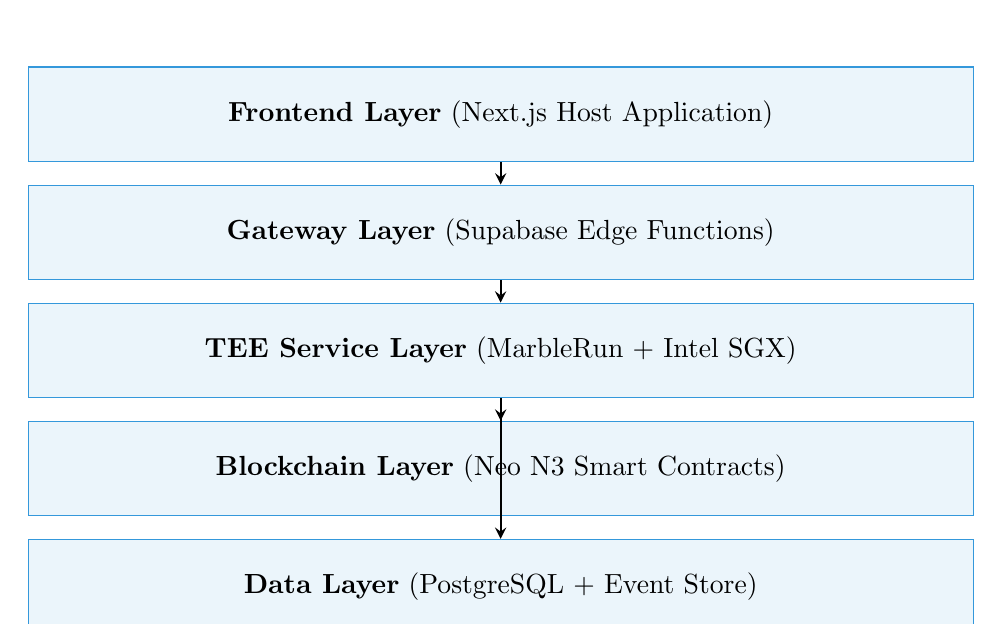
\begin{tikzpicture}[
    layer/.style={rectangle, draw=neoblue, fill=neoblue!10, minimum width=12cm, minimum height=1.2cm, align=center},
    arrow/.style={->, thick, >=stealth}
]
    \node[layer] (frontend) at (0,6) {\textbf{Frontend Layer} (Next.js Host Application)};
    \node[layer] (gateway) at (0,4.5) {\textbf{Gateway Layer} (Supabase Edge Functions)};
    \node[layer] (tee) at (0,3) {\textbf{TEE Service Layer} (MarbleRun + Intel SGX)};
    \node[layer] (blockchain) at (0,1.5) {\textbf{Blockchain Layer} (Neo N3 Smart Contracts)};
    \node[layer] (data) at (0,0) {\textbf{Data Layer} (PostgreSQL + Event Store)};

    \draw[arrow] (frontend) -- (gateway);
    \draw[arrow] (gateway) -- (tee);
    \draw[arrow] (tee) -- (blockchain);
    \draw[arrow] (tee) -- (data);
\end{tikzpicture}
\caption{Neo N3 MiniApp Platform Architecture}
\end{figure}

\subsection{Frontend Layer}

The Frontend Layer serves as the primary interface between users and the platform, implementing a host application architecture that functions as an ``app store'' for MiniApps. Built on Next.js and deployed via Vercel's edge network, this layer provides global low-latency access while maintaining strict security boundaries between the host application and individual MiniApps.

MiniApp isolation is achieved through two complementary mechanisms. For maximum security, MiniApps execute within sandboxed iframes with restrictive Content Security Policies that prevent cross-origin data access and script injection. For performance-critical applications requiring tighter integration, Webpack Module Federation enables controlled code sharing while maintaining logical separation. The host application manages authentication state through Supabase Auth, providing OAuth-based user onboarding that eliminates the need for blockchain-specific wallet creation during initial registration.

The Frontend Layer implements a bridge protocol that enables secure communication between MiniApps and platform services. This bridge validates all requests against the MiniApp's declared manifest permissions, ensuring that applications cannot exceed their authorized capabilities. The bridge also manages the lifecycle of user sessions, handling token refresh, session persistence, and graceful degradation when network connectivity is interrupted.

\subsection{Gateway Layer}

The Gateway Layer, implemented as Supabase Edge Functions, provides a stateless routing and validation layer that mediates all communication between the Frontend Layer and backend services. This layer executes at the network edge, minimizing latency while providing consistent security enforcement regardless of user geographic location.

Authentication and authorization represent the primary responsibilities of the Gateway Layer. Every request undergoes JWT validation to verify user identity, followed by rate limiting to prevent abuse and ensure fair resource allocation across users. The Gateway Layer validates all requests against the originating MiniApp's manifest, ensuring that requested operations fall within declared permissions and resource limits. For payment operations, the Gateway Layer enforces the platform's GAS-only policy, rejecting any attempt to process non-GAS assets before requests reach backend services.

Communication between the Gateway Layer and TEE services occurs over mutual TLS (mTLS) connections, ensuring that only authenticated gateway instances can invoke sensitive backend operations. This architecture prevents direct access to TEE services from external networks, establishing the Gateway Layer as a mandatory security checkpoint for all platform interactions.

\subsection{TEE Service Layer}

The Trusted Execution Environment Service Layer represents the security foundation of the Neo N3 MiniApp Platform, providing hardware-protected execution for all sensitive operations. This layer leverages Intel Software Guard Extensions (SGX) technology through the EGo framework, with MarbleRun providing orchestration, attestation, and secure secret distribution across enclave instances.

Within this layer, six specialized services handle distinct categories of sensitive operations. The NeoFeeds service aggregates price data from multiple external sources, computing median values within the enclave to prevent manipulation. The NeoVRF service generates cryptographically secure random numbers using enclave-protected signing keys, with optional on-chain anchoring for verifiable randomness. The NeoOracle service fetches external data from allowlisted endpoints, injecting secrets securely using AES-GCM encryption. The NeoCompute service executes restricted JavaScript code within the enclave, enabling confidential computation with encrypted outputs. The NeoFlow service manages task scheduling and automation triggers, anchoring execution proofs on-chain. The TxProxy service handles transaction construction and signing, enforcing policy constraints before submitting transactions to the Neo N3 network.

Key material within the TEE Service Layer is bound to specific enclave measurements through SGX sealing, ensuring that keys cannot be extracted even by privileged system software. MarbleRun's manifest-based configuration defines the expected measurements for each service, enabling remote attestation that verifies enclave integrity before secrets are provisioned.

\subsection{Blockchain Layer}

The Blockchain Layer comprises seven smart contracts deployed on the Neo N3 network, providing immutable enforcement of platform rules and serving as the final authority for all financial and governance operations. These contracts are designed with minimal complexity to reduce attack surface while providing comprehensive functionality for platform operations.

The PaymentHub contract serves as the central settlement mechanism, processing all GAS payments and distributing revenue between MiniApp developers and the platform treasury. This contract implements strict asset validation, rejecting any non-GAS tokens at the contract level to ensure compliance with platform policies. The Governance contract manages NEO staking and proposal voting, enabling token holders to participate in platform governance decisions. The PriceFeed contract stores oracle price data with TEE attestation signatures, providing on-chain price references for DeFi applications. The RandomnessLog contract anchors verifiable random values generated by the NeoVRF service, enabling on-chain verification of randomness used in gaming applications. The AppRegistry contract maintains the registry of approved MiniApps, storing manifest hashes and managing the allowlist of authorized applications. The AutomationAnchor contract records task execution proofs from the NeoFlow service, providing anti-replay protection for automated operations. The ServiceLayerGateway contract routes on-chain service requests to appropriate TEE services, enabling smart contracts to invoke platform capabilities.

\subsection{Data Layer}

The Data Layer provides persistent storage for platform state that does not require blockchain immutability, utilizing Supabase's managed PostgreSQL infrastructure with row-level security policies. This layer stores user profiles, session data, MiniApp analytics, and event logs, enabling rich querying capabilities that would be impractical on-chain.

\begin{figure}[h]
\centering
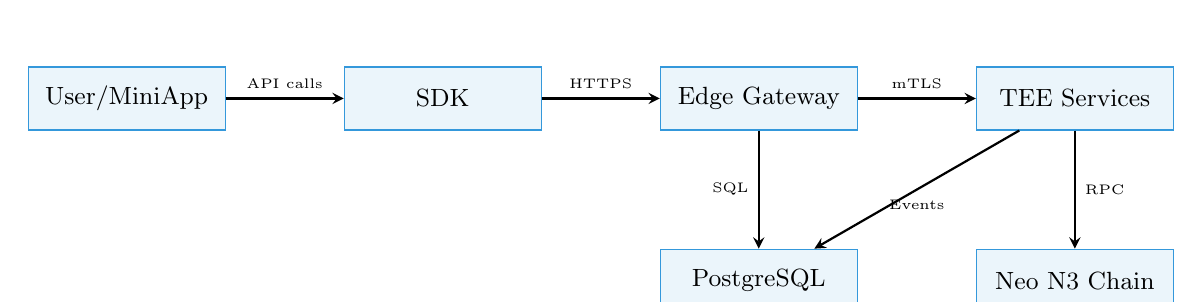
\begin{tikzpicture}[
    node distance=1.5cm,
    box/.style={rectangle, draw=neoblue, fill=neoblue!10, minimum width=2.5cm, minimum height=0.8cm, align=center, font=\small},
    arrow/.style={->, thick, >=stealth}
]
    % Nodes
    \node[box] (user) {User/MiniApp};
    \node[box, right=of user] (sdk) {SDK};
    \node[box, right=of sdk] (edge) {Edge Gateway};
    \node[box, right=of edge] (tee) {TEE Services};
    \node[box, below=of tee] (chain) {Neo N3 Chain};
    \node[box, below=of edge] (db) {PostgreSQL};

    % Arrows
    \draw[arrow] (user) -- node[above, font=\tiny] {API calls} (sdk);
    \draw[arrow] (sdk) -- node[above, font=\tiny] {HTTPS} (edge);
    \draw[arrow] (edge) -- node[above, font=\tiny] {mTLS} (tee);
    \draw[arrow] (tee) -- node[right, font=\tiny] {RPC} (chain);
    \draw[arrow] (edge) -- node[left, font=\tiny] {SQL} (db);
    \draw[arrow] (tee) -- node[below, font=\tiny] {Events} (db);
\end{tikzpicture}
\caption{Platform Data Flow Architecture}
\label{fig:data-flow}
\end{figure}

Event sourcing patterns capture all significant platform events, creating an immutable audit trail that complements on-chain transaction records. This event store enables reconstruction of platform state at any historical point, supporting debugging, compliance reporting, and analytics. Real-time subscriptions through Supabase's PostgreSQL NOTIFY mechanism enable instant updates to connected clients when relevant events occur, supporting responsive user interfaces without polling.

\newpage
%==============================================================================
% SECTION 3: SECURITY MODEL
%==============================================================================
\section{Security Model}

\subsection{Defense in Depth Architecture}

The Neo N3 MiniApp Platform implements a defense-in-depth security architecture comprising four distinct enforcement layers. This approach ensures that security is not dependent on any single mechanism, providing resilience against both known attack vectors and novel threats. Each layer implements independent validation logic, ensuring that a compromise at one layer does not automatically propagate to others.

\begin{table}[h]
\centering
\caption{Defense-in-Depth Security Layers}
\begin{tabular}{@{}llll@{}}
\toprule
\textbf{Layer} & \textbf{Location} & \textbf{Primary Function} & \textbf{Trust Level} \\
\midrule
Layer 1 & Client SDK & Input validation, type checking & Untrusted \\
Layer 2 & Edge Gateway & Auth, rate limiting, schema validation & Trusted \\
Layer 3 & TEE Services & Cryptographic ops, business logic & Hardware-protected \\
Layer 4 & Smart Contracts & Immutable rule enforcement & Blockchain-secured \\
\bottomrule
\end{tabular}
\label{tab:security-layers}
\end{table}

The first layer of defense resides within the client-side SDK, which performs input validation, type checking, and preliminary constraint enforcement before requests leave the user's device. While client-side validation cannot be trusted for security enforcement, it provides immediate feedback to users and developers, catching common errors before they consume network resources. The SDK also implements rate limiting awareness, preventing applications from exceeding their allocated request quotas.

The second layer operates at the Edge Gateway, where server-side validation occurs in a controlled environment. This layer authenticates users through JWT verification, enforces rate limits through distributed counters, validates request schemas against expected formats, and verifies that requested operations comply with the originating MiniApp's manifest permissions. The Gateway Layer represents the first trusted enforcement point, as it operates on infrastructure controlled by the platform.

The third layer executes within Trusted Execution Environments, where the most sensitive operations occur. TEE services validate all inputs against expected formats and ranges, enforce business logic constraints, and perform cryptographic operations using enclave-protected keys. The hardware isolation provided by Intel SGX ensures that even privileged system software cannot observe or manipulate operations within the enclave.

The fourth and final layer resides in on-chain smart contracts, which provide immutable enforcement of critical rules. Smart contracts validate transaction parameters, enforce asset type restrictions, and maintain authoritative state that cannot be modified except through valid transactions. This layer serves as the ultimate arbiter of platform rules, providing guarantees that persist even if all other layers are compromised.

\subsection{Asset Separation and Compliance}

The platform enforces strict separation between utility and governance tokens, mandating GAS for all payment operations and NEO for all governance activities. This separation serves multiple purposes: it ensures clear utility for each token type, simplifies regulatory compliance by maintaining distinct asset classes, and aligns stakeholder incentives by requiring governance participation to hold governance tokens.

Asset separation is enforced at every layer of the platform architecture. The SDK rejects attempts to construct payment transactions with non-GAS assets, providing immediate developer feedback. The Gateway Layer validates asset types in all payment requests, rejecting non-compliant requests before they reach backend services. TEE services verify asset types before constructing transactions, ensuring that even compromised gateway instances cannot bypass restrictions. Finally, the PaymentHub smart contract implements on-chain asset validation, rejecting any non-GAS transfers at the contract level.

This multi-layer enforcement ensures that asset separation cannot be circumvented through any single point of compromise. An attacker would need to simultaneously compromise the SDK distribution, gateway infrastructure, TEE services, and smart contract logic to process unauthorized asset types---a practically infeasible attack scenario.

\subsection{Trusted Execution Environment Security}

Intel SGX technology provides the hardware foundation for the platform's security model, enabling code execution within isolated enclaves that are protected from observation or manipulation by any software running outside the enclave, including the operating system and hypervisor. This protection extends to physical attacks, as enclave memory is encrypted by the CPU using keys that are not accessible to any external entity.

The platform leverages SGX through the EGo framework, which enables Go applications to execute within SGX enclaves with minimal modification. MarbleRun provides orchestration and attestation services, managing the lifecycle of enclave instances and ensuring that secrets are only provisioned to enclaves with expected measurements. The MarbleRun manifest defines the expected code measurements, signing keys, and configuration parameters for each service, enabling remote verification of enclave integrity.

Key management within TEE services follows a hierarchical derivation model. A master key, generated within the enclave during initial provisioning, is sealed to the enclave measurement using SGX sealing. Service-specific keys are derived from this master key using domain separation, ensuring that compromise of one service's keys does not affect others. Transaction signing keys are further derived per-account, enabling fine-grained access control and key rotation without affecting other accounts.

Side-channel attack mitigations are implemented throughout TEE services, including constant-time cryptographic operations, memory access pattern obfuscation, and careful management of enclave entry and exit points. While SGX provides strong isolation guarantees, the platform's security model does not rely solely on SGX, instead treating TEE protection as one layer within the broader defense-in-depth architecture.

\subsection{Account Pool Security}

The account pool architecture presents unique security considerations, as the platform maintains custody of private keys for over ten thousand pre-generated accounts. These keys are generated within TEE enclaves using hardware random number generators, ensuring that key material is never exposed outside protected memory.

Account keys are stored in encrypted form using SGX sealing, with the sealing key bound to the specific enclave measurement. This ensures that account keys can only be decrypted by enclave instances running the expected code version. Key rotation is supported through a migration protocol that re-encrypts keys under new sealing keys when enclave code is updated.

Access to account pool operations is restricted through multiple mechanisms. Service authentication via mTLS ensures that only authorized services can request account operations. Per-service quotas limit the rate at which accounts can be requested, preventing resource exhaustion attacks. Audit logging captures all account operations, enabling detection of anomalous access patterns. Finally, account locking mechanisms prevent concurrent use of the same account, ensuring transaction ordering consistency.

\newpage
%==============================================================================
% SECTION 4: CORE SERVICES
%==============================================================================
\section{Core Services}

The Neo N3 MiniApp Platform provides six specialized services that execute within Trusted Execution Environments, each designed to address specific categories of sensitive operations that MiniApps require. These services form the operational backbone of the platform, enabling applications to access price data, generate verifiable randomness, fetch external information, execute confidential computations, automate workflows, and submit blockchain transactions---all within the security guarantees provided by hardware-protected enclaves.

\begin{table}[h]
\centering
\caption{TEE Services Overview}
\begin{tabular}{@{}lll@{}}
\toprule
\textbf{Service} & \textbf{Primary Function} & \textbf{On-Chain Anchor} \\
\midrule
NeoFeeds & Price data aggregation & PriceFeed contract \\
NeoVRF & Verifiable randomness & RandomnessLog contract \\
NeoOracle & External data fetching & Optional callback \\
NeoCompute & Confidential computation & Encrypted output \\
NeoFlow & Workflow automation & AutomationAnchor contract \\
TxProxy & Transaction signing & Neo N3 network \\
\bottomrule
\end{tabular}
\label{tab:tee-services}
\end{table}

\subsection{NeoFeeds: Real-Time Price Data Aggregation}

The NeoFeeds service addresses the critical requirement for reliable, manipulation-resistant price data that underpins decentralized finance applications. Traditional oracle solutions face challenges including single points of failure, data manipulation by malicious sources, and latency in price updates. NeoFeeds mitigates these risks through multi-source aggregation within a trusted execution environment.

The service continuously polls price data from multiple independent sources, including centralized exchanges, decentralized exchanges, and professional data providers. Within the SGX enclave, the service computes median values across sources, effectively filtering outliers and preventing any single source from manipulating reported prices. A configurable deviation threshold, defaulting to 0.1\%, determines when price updates warrant on-chain anchoring, balancing data freshness against transaction costs.

Price data is anchored on-chain through the PriceFeed smart contract, accompanied by TEE attestation signatures that enable consumers to verify data authenticity. This architecture ensures that even if external data sources are compromised, the aggregation logic within the enclave provides resilience against manipulation, while on-chain anchoring creates an immutable record of historical prices.

\subsection{NeoVRF: Verifiable Random Function Service}

Randomness represents a fundamental primitive for gaming, lottery, and fair selection applications, yet generating truly unpredictable random values in deterministic blockchain environments presents significant challenges. The NeoVRF service provides cryptographically secure randomness through a Verifiable Random Function implementation that executes within the TEE.

The service generates random values using enclave-protected signing keys, producing outputs that are both unpredictable before generation and verifiable after the fact. Each random value is accompanied by a proof that enables any party to verify that the output was correctly derived from the input seed and the service's public key, without revealing the private key used in generation.

For applications requiring on-chain verifiability, NeoVRF supports optional anchoring through the RandomnessLog contract. This anchoring creates an immutable record of generated random values, enabling smart contracts to verify randomness used in gaming outcomes or lottery drawings. The attestation hash included with each random value provides cryptographic proof that the value was generated within a valid TEE instance.

\subsection{NeoOracle: Confidential External Data Access}

Many blockchain applications require access to external data sources, from weather information for parametric insurance to sports scores for prediction markets. The NeoOracle service enables secure fetching of external data while protecting sensitive credentials and API keys from exposure.

The service maintains an allowlist of approved HTTP endpoints, preventing arbitrary network access that could be exploited for malicious purposes. When fetching data, the service can inject secrets---such as API keys or authentication tokens---using AES-GCM encryption, ensuring that credentials are never exposed outside the enclave. Per-secret permission enforcement ensures that each MiniApp can only access secrets explicitly granted to it.

Data fetched through NeoOracle is processed within the enclave before being returned to requesting applications. This processing can include parsing, validation, and transformation, ensuring that applications receive clean, structured data. The enclave's isolation guarantees that sensitive credentials cannot be extracted even by privileged system administrators.

\subsection{NeoCompute: Confidential Code Execution}

Certain application logic requires confidentiality guarantees that cannot be achieved through on-chain execution, where all computation is publicly visible. The NeoCompute service enables execution of restricted JavaScript code within the TEE, providing confidential computation capabilities for sensitive business logic.

The service accepts JavaScript code along with input parameters, executing the code within a sandboxed environment inside the enclave. Configurable timeouts and resource limits prevent denial-of-service attacks through resource exhaustion. The execution environment provides access to cryptographic primitives and utility functions while restricting network access and file system operations.

Computation outputs are encrypted using keys derived from the requesting application's identity, ensuring that results can only be decrypted by authorized parties. Each output includes a signature from the enclave's attestation key, enabling verification that the computation occurred within a valid TEE instance. This architecture enables applications to implement confidential business logic---such as sealed-bid auctions or private matching algorithms---while maintaining verifiability.

\subsection{NeoFlow: Workflow Automation and Scheduling}

Blockchain applications often require automated execution of recurring tasks or triggered responses to external events. The NeoFlow service provides workflow automation capabilities, enabling MiniApps to schedule tasks and define triggers without maintaining dedicated infrastructure.

The service supports cron-based scheduling for recurring tasks, enabling applications to perform periodic operations such as daily settlements, weekly distributions, or hourly data updates. Price-based triggers enable reactive automation, executing specified actions when asset prices cross defined thresholds. All scheduled executions are anchored on-chain through the AutomationAnchor contract, providing anti-replay protection and creating an auditable record of automated operations.

Task definitions are stored within the TEE, ensuring that automation logic cannot be observed or manipulated by external parties. The service manages task lifecycle, including creation, modification, suspension, and deletion, with all operations authenticated against the requesting application's identity.

\subsection{TxProxy: Transaction Construction and Signing}

The TxProxy service serves as the gateway between platform services and the Neo N3 blockchain, handling transaction construction, signing, and submission. This service implements the platform's transaction policies, ensuring that all blockchain interactions comply with defined constraints.

Before constructing any transaction, TxProxy validates the request against multiple policy layers. Contract allowlists ensure that transactions can only interact with approved smart contracts. Method restrictions limit which contract methods can be invoked. Amount limits cap the value that can be transferred in single transactions. Intent gates require explicit user confirmation for high-value or sensitive operations.

Transaction signing occurs using keys from the account pool, with key selection based on the requesting service and operation type. The service manages transaction lifecycle, including nonce management, fee estimation, submission, and confirmation monitoring. Failed transactions are automatically retried with adjusted parameters, while persistent failures are reported to requesting services for appropriate handling.

\newpage
%==============================================================================
% SECTION 5: SMART CONTRACTS
%==============================================================================
\section{Smart Contract Infrastructure}

The blockchain layer of the Neo N3 MiniApp Platform comprises seven carefully designed smart contracts that provide immutable enforcement of platform rules and serve as the authoritative source of truth for all financial and governance operations. These contracts are implemented in C\# using the Neo N3 smart contract framework, leveraging the platform's native support for complex data structures and efficient execution.

\begin{table}[h]
\centering
\caption{Platform Smart Contracts}
\begin{tabular}{@{}llp{5.5cm}@{}}
\toprule
\textbf{Contract} & \textbf{Asset Policy} & \textbf{Primary Function} \\
\midrule
PaymentHub & GAS only & Payment settlement and revenue distribution \\
Governance & NEO only & Staking, proposals, and voting \\
PriceFeed & N/A & Oracle price data with TEE attestation \\
RandomnessLog & N/A & VRF randomness anchoring \\
AppRegistry & N/A & MiniApp registration and allowlist \\
AutomationAnchor & N/A & Task execution proofs \\
ServiceLayerGateway & GAS (fees) & On-chain service request routing \\
\bottomrule
\end{tabular}
\label{tab:smart-contracts}
\end{table}

\begin{table}[h]
\centering
\caption{Platform Contract Addresses (Neo N3 Testnet)}
\begin{tabular}{@{}ll@{}}
\toprule
\textbf{Contract} & \textbf{Address} \\
\midrule
PaymentHub & \texttt{NZLGNdQUa5jQ2VC1r3MGoJFGm3BW8Kv81q} \\
Governance & \texttt{NLRGStjsRpN3bk71KNoKe74fNxUT72gfpe} \\
PriceFeed & \texttt{NTdJ7XHZtYXSRXnWGxV6TcyxiSRCcjP4X1} \\
RandomnessLog & \texttt{NR9urKR3FZqAfvowx2fyWjtWHBpqLqrEPP} \\
AppRegistry & \texttt{NXZNTXiPuBRHnEaKFV3tLHhitkbt3XmoWJ} \\
AutomationAnchor & \texttt{NcVrd4Z7W8sxv9jvdBF72xfiWBnvRsgVkx} \\
ServiceLayerGateway & \texttt{NTWh6auSz3nvBZSbXHbZz4ShwPhmpkC5Ad} \\
\bottomrule
\end{tabular}
\label{tab:platform-contracts-addresses}
\end{table}

\subsection{PaymentHub: Central Settlement Mechanism}

The PaymentHub contract serves as the financial backbone of the platform, processing all GAS payments between users, MiniApps, and the platform treasury. This contract implements the platform's strict GAS-only policy at the most fundamental level, providing guarantees that cannot be circumvented regardless of the state of other system components.

When a payment is initiated, the PaymentHub contract first validates that the incoming asset is GAS, rejecting any other token type with an explicit error. The contract then records the payment details, including the source address, destination MiniApp, amount, and memo field. Revenue distribution occurs according to configurable split ratios, automatically allocating portions to the MiniApp developer, platform treasury, and governance reward pool.

The contract maintains comprehensive audit trails for all transactions, enabling reconstruction of payment history for compliance reporting and dispute resolution. Event emissions notify off-chain systems of payment completions, enabling real-time updates to user interfaces and analytics dashboards.

\subsection{Governance: Stakeholder Participation}

The Governance contract enables NEO token holders to participate in platform decision-making through a structured proposal and voting mechanism. This contract enforces the platform's NEO-only governance policy, ensuring that voting power is proportional to governance token holdings.

Proposals follow a defined lifecycle: creation, discussion period, voting period, and execution. During the voting period, NEO holders can cast votes weighted by their token balance at a snapshot block height, preventing vote manipulation through last-minute token transfers. Quorum requirements ensure that proposals cannot pass without sufficient participation, while supermajority thresholds protect against contentious changes.

The contract supports delegation, enabling token holders to assign their voting power to trusted representatives without transferring token custody. Delegation can be revoked at any time, and delegated votes are automatically updated when the delegator's balance changes.

\subsection{PriceFeed: Oracle Data Anchoring}

The PriceFeed contract stores price data submitted by the NeoFeeds TEE service, creating an on-chain record of asset prices that can be consumed by other smart contracts. Each price update includes the asset pair, price value, timestamp, and TEE attestation signature.

Before accepting a price update, the contract validates the attestation signature against the registered TEE public key, ensuring that only authorized enclave instances can submit price data. The contract maintains historical price records, enabling queries for prices at specific timestamps and calculation of time-weighted average prices.

Price consumers can query current prices directly or subscribe to price update events for real-time notifications. The contract implements staleness checks, returning errors when requested prices exceed configurable age thresholds, preventing applications from acting on outdated information.

\subsection{RandomnessLog: Verifiable Randomness Anchoring}

The RandomnessLog contract provides on-chain anchoring for random values generated by the NeoVRF service, enabling smart contracts to verify that randomness used in gaming or selection applications was generated correctly. Each anchored random value includes the input seed, output value, and VRF proof.

Verification functions enable any party to confirm that an anchored random value was correctly derived from its seed using the registered VRF public key. This verification can occur on-chain within other smart contracts or off-chain by interested parties, providing transparency for gaming applications.

The contract maintains an index of random values by request identifier, enabling efficient lookup of randomness associated with specific application operations. Historical queries support audit and compliance requirements for gaming applications subject to regulatory oversight.

\subsection{AppRegistry: Application Management}

The AppRegistry contract maintains the authoritative registry of approved MiniApps, storing manifest hashes and managing the allowlist of applications authorized to operate on the platform. This contract serves as the gatekeeper for platform access, ensuring that only vetted applications can interact with platform services.

Each registered application entry includes the application identifier, manifest hash, developer address, registration timestamp, and status flags. The manifest hash enables verification that an application's declared permissions and constraints match the version reviewed during the approval process. Any modification to an application's manifest requires re-registration with an updated hash.

The contract implements role-based access control for administrative operations, with separate roles for application registration, status modification, and configuration updates. Multi-signature requirements for sensitive operations prevent unilateral changes by compromised administrator accounts.

\subsection{AutomationAnchor: Task Execution Proofs}

The AutomationAnchor contract records execution proofs for automated tasks managed by the NeoFlow service, providing anti-replay protection and creating an auditable record of automated operations. Each execution record includes the task identifier, execution timestamp, input parameters hash, and TEE attestation.

Anti-replay protection ensures that each task execution can only be recorded once, preventing duplicate processing of automated operations. The contract validates attestation signatures before accepting execution records, ensuring that only authorized TEE instances can submit proofs.

Historical queries enable reconstruction of automation execution history, supporting debugging and compliance requirements. The contract emits events for each recorded execution, enabling off-chain systems to track automation activity in real-time.

\subsection{ServiceLayerGateway: On-Chain Service Routing}

The ServiceLayerGateway contract enables smart contracts to invoke platform services through on-chain requests, bridging the gap between on-chain logic and off-chain TEE services. This contract implements a request-callback pattern that maintains the security properties of both on-chain and off-chain execution.

When a smart contract submits a service request, the gateway contract validates the request parameters and emits an event that TEE services monitor. The appropriate service processes the request within its enclave and submits the result back to the gateway contract, which routes the response to the original requesting contract through a callback mechanism.

Request authentication ensures that only authorized contracts can invoke specific services, with per-service access control lists managed by platform administrators. Fee handling collects GAS payments for service invocations, distributing fees according to platform revenue sharing policies.

\newpage
%==============================================================================
% SECTION 6: BUILT-IN MINIAPPS
%==============================================================================
\section{Built-in MiniApps}

The Neo N3 MiniApp Platform includes twenty-three production-ready applications that demonstrate platform capabilities while providing immediate utility to users. These built-in MiniApps span four primary categories---gaming, decentralized finance, social interaction, and governance---each showcasing different aspects of the platform's technical capabilities.

\begin{table}[h]
\centering
\caption{Built-in MiniApps by Category}
\begin{tabular}{@{}llp{6cm}@{}}
\toprule
\textbf{Category} & \textbf{Application} & \textbf{Description} \\
\midrule
\multirow{7}{*}{Gaming} & Neo Lottery & Ticket-based lottery with VRF selection \\
 & Coin Flip & Double-or-nothing wagering \\
 & Dice Game & Variable multiplier dice rolls \\
 & Scratch Card & Instant-win experiences \\
 & Gas Spin & Wheel-of-fortune mechanics \\
 & Secret Poker & TEE-protected Texas Hold'em \\
 & Fog Chess & Information asymmetry chess \\
\midrule
\multirow{6}{*}{DeFi} & Prediction Market & Price movement betting \\
 & Flash Loan & Instant borrow-and-repay \\
 & Price Ticker & Real-time price feeds \\
 & AI Trader & Autonomous trading strategies \\
 & Grid Bot & Automated grid trading \\
 & IL Guard & Impermanent loss protection \\
\midrule
\multirow{4}{*}{Social} & Red Envelope & WeChat-style lucky packets with best luck winner \\
 & Gas Circle & Rotating savings circles \\
 & Secret Vote & Privacy-preserving voting \\
 & NFT Evolve & Dynamic NFT mechanics \\
\midrule
\multirow{3}{*}{Governance} & Gov Booster & NEO governance optimization \\
 & Bridge Guardian & Cross-chain transfers \\
 & Guardian Policy & TEE transaction security \\
\bottomrule
\end{tabular}
\label{tab:miniapps}
\end{table}

\begin{table}[h]
\centering
\caption{MiniApp Contract Addresses (Neo N3 Testnet)}
\scriptsize
\begin{tabular}{@{}lll@{}}
\toprule
\textbf{Category} & \textbf{Contract} & \textbf{Script Hash} \\
\midrule
\multirow{6}{*}{Gaming} & MiniAppLottery & \texttt{0x3e330b4c396b40aa08d49912c0179319831b3a6e} \\
 & MiniAppCoinFlip & \texttt{0xbd4c9203495048900e34cd9c4618c05994e86cc0} \\
 & MiniAppDiceGame & \texttt{0xfacff9abd201dca86e6a63acfb5d60da278da8ea} \\
 & MiniAppScratchCard & \texttt{0x2674ef3b4d8c006201d1e7e473316592f6cde5f2} \\
 & MiniAppSecretPoker & \texttt{0xa27348cc0a79c776699a028244250b4f3d6bbe0c} \\
 & MiniAppFogChess & \texttt{0x23a44ca6643c104fbaa97daab65d5e53b3662b4a} \\
\bottomrule
\end{tabular}
\label{tab:miniapps-gaming-addresses}
\end{table}

\begin{table}[h]
\centering
\caption{MiniApp Contract Addresses - DeFi (Neo N3 Testnet)}
\scriptsize
\begin{tabular}{@{}ll@{}}
\toprule
\textbf{Contract} & \textbf{Script Hash} \\
\midrule
MiniAppPredictionMarket & \texttt{0x64118096bd004a2bcb010f4371aba45121eca790} \\
MiniAppFlashLoan & \texttt{0xee51e5b399f7727267b7d296ff34ec6bb9283131} \\
MiniAppPriceTicker & \texttt{0x838bd5dd3d257a844fadddb5af2b9dac45e1d320} \\
MiniAppILGuard & \texttt{0xd3557ccbb2ced2254f5862fbc784cd97cf746872} \\
MiniAppAITrader & \texttt{0xc3356f394897e36b3903ea81d87717da8db98809} \\
MiniAppGridBot & \texttt{0x0d9cfc40ac2ab58de449950725af9637e0884b28} \\
\bottomrule
\end{tabular}
\label{tab:miniapps-defi-addresses}
\end{table}

\begin{table}[h]
\centering
\caption{MiniApp Contract Addresses - Social \& Governance (Neo N3 Testnet)}
\scriptsize
\begin{tabular}{@{}lll@{}}
\toprule
\textbf{Category} & \textbf{Contract} & \textbf{Script Hash} \\
\midrule
\multirow{4}{*}{Social} & MiniAppRedEnvelope & \texttt{0xf2649c2b6312d8c7b4982c0c597c9772a2595b1e} \\
 & MiniAppGasCircle & \texttt{0x7736c8d1ff918f94d26adc688dac4d4bc084bd39} \\
 & MiniAppSecretVote & \texttt{0x7763ce957515f6acef6d093376977ac6c1cbc47d} \\
 & MiniAppNFTEvolve & \texttt{0xadd18a719d14d59c064244833cd2c812c79d6015} \\
\midrule
\multirow{3}{*}{Governance} & MiniAppGovBooster & \texttt{0xebabd9712f985afc0e5a4e24ed2fc4acb874796f} \\
 & MiniAppBridgeGuardian & \texttt{0x2d03f3e4ff10e14ea94081e0c21e79e79c33f9e3} \\
 & MiniAppGuardianPolicy & \texttt{0x893a774957244b83a0efed1d42771fe1e424cfec} \\
\bottomrule
\end{tabular}
\label{tab:miniapps-social-gov-addresses}
\end{table}

\subsection{Gaming Applications}

The gaming category comprises seven applications that leverage the platform's verifiable randomness and payment infrastructure to deliver provably fair gaming experiences. These applications demonstrate how traditional gaming mechanics can be implemented with blockchain-backed fairness guarantees.

The Neo Lottery application implements a ticket-based lottery system where users purchase tickets using GAS tokens, with winners selected through verifiable random number generation. Each lottery round accumulates a prize pool from ticket sales, with the NeoVRF service generating the winning ticket number at the conclusion of each round. The on-chain anchoring of random values enables any participant to verify that winner selection was fair and unmanipulated.

The Coin Flip application provides a simple double-or-nothing game where users wager GAS on the outcome of a virtual coin flip. The application demonstrates the platform's ability to deliver instant gaming experiences, with randomness generation and payout processing completing within seconds. The 50/50 odds are mathematically verifiable through the VRF proof mechanism.

The Dice Game application extends the multiplier concept, allowing users to bet on dice roll outcomes with payouts up to six times the wager amount. Variable odds based on the selected number range demonstrate how the platform supports complex payout structures while maintaining provable fairness.

Additional gaming applications include Scratch Card for instant-win experiences, Gas Spin for wheel-of-fortune mechanics, Secret Poker for Texas Hold'em with TEE-protected hidden cards, and Fog Chess for strategic gameplay with information asymmetry enforced by the trusted execution environment.

\subsection{Decentralized Finance Applications}

The DeFi category includes nine applications that demonstrate the platform's capabilities for financial applications, from simple price queries to sophisticated trading strategies. These applications leverage the NeoFeeds price oracle and payment infrastructure to deliver financial services within the platform's security model.

The Prediction Market application enables users to bet on future price movements of supported asset pairs. Users take positions on whether prices will rise or fall within specified timeframes, with outcomes determined by price data from the NeoFeeds oracle. The application demonstrates how external data can be securely incorporated into on-chain settlement logic.

The Flash Loan application implements instant borrow-and-repay mechanics, enabling users to access liquidity for arbitrage or other operations that complete within a single transaction. The application enforces repayment within the same transaction, eliminating default risk while enabling capital-efficient operations.

The Price Ticker application provides real-time price feeds for supported asset pairs, demonstrating the NeoFeeds oracle integration. Users can query current prices and subscribe to price update notifications, enabling informed trading decisions based on reliable market data.

Additional DeFi applications include Price Predict and Micro Predict for binary options trading at different timeframes, Turbo Options for ultra-fast trading, IL Guard for impermanent loss protection, AI Trader for autonomous trading strategies, and Grid Bot for automated grid trading.

\subsection{Social and Governance Applications}

The social and governance category encompasses seven applications that facilitate community interaction and platform governance. These applications demonstrate how blockchain technology can enhance social coordination and democratic decision-making.

The Red Envelope application implements WeChat-style lucky red packets, enabling users to create GAS-filled envelopes that recipients can claim with random amounts. Unlike equal distribution, each recipient receives a different VRF-generated random amount, creating excitement as users discover their luck. The application tracks all grabbers and their amounts, preventing duplicate claims from the same user. When all packets are claimed, the person who received the highest amount is crowned the ``Best Luck Winner'', with a platform notification announcing the winner to all participants. The smart contract is deployed on Neo N3 Testnet at \texttt{0xf2649c2b6312d8c7b4982c0c597c9772a2595b1e}.

The Gas Circle application creates daily savings circles where participants contribute GAS to a shared pool, with one member receiving the accumulated funds each cycle. The application demonstrates how traditional rotating savings mechanisms can be implemented with blockchain-backed transparency and enforcement.

The Secret Vote application enables privacy-preserving voting for community decisions, leveraging the TEE to ensure that individual votes remain confidential while producing verifiable aggregate results. This application demonstrates how the platform's confidential computing capabilities can protect voter privacy in governance contexts.

The Gov Booster application provides tools for NEO governance optimization, helping token holders maximize their participation in Neo network governance. Additional applications include NFT Evolve for dynamic NFT mechanics, Bridge Guardian for cross-chain asset transfers, and Guardian Policy for TEE-enforced transaction security policies.

\newpage
%==============================================================================
% SECTION 7: DEVELOPER GUIDE
%==============================================================================
\section{Developer Guide}

The Neo N3 MiniApp Platform provides comprehensive tooling and documentation to enable developers to build, test, and deploy MiniApps efficiently. This section outlines the development workflow, SDK capabilities, and manifest specification that govern MiniApp behavior.

\subsection{Development Environment}

Developers begin by installing the platform SDK, which provides TypeScript bindings for all platform services. The SDK is distributed through npm and can be installed with a single command. Once installed, developers have access to typed interfaces for payments, randomness, price feeds, governance, and other platform capabilities.

The SDK implements automatic environment detection, configuring itself for testnet or mainnet based on initialization parameters. During development, applications can operate against a local simulation environment that mimics platform behavior without requiring blockchain transactions, enabling rapid iteration and testing.

\subsection{SDK Architecture}

The SDK exposes platform capabilities through a modular architecture, with separate namespaces for different service categories. The payments namespace provides methods for initiating GAS transfers, querying balances, and subscribing to payment events. The randomness namespace enables requesting verifiable random values with configurable anchoring options. The datafeed namespace provides access to price oracle data with support for historical queries and real-time subscriptions.

\begin{table}[h]
\centering
\caption{SDK Namespace Overview}
\begin{tabular}{@{}lp{7cm}@{}}
\toprule
\textbf{Namespace} & \textbf{Key Methods} \\
\midrule
\texttt{wallet} & \texttt{getAddress()}, \texttt{bindWallet()} \\
\texttt{payments} & \texttt{payGAS()}, \texttt{getBalance()}, \texttt{subscribe()} \\
\texttt{rng} & \texttt{requestRandom()}, \texttt{verifyProof()} \\
\texttt{datafeed} & \texttt{getPrice()}, \texttt{subscribe()}, \texttt{getHistory()} \\
\texttt{governance} & \texttt{vote()}, \texttt{stake()}, \texttt{delegate()} \\
\texttt{stats} & \texttt{getMyUsage()}, \texttt{getAppStats()} \\
\bottomrule
\end{tabular}
\label{tab:sdk-namespaces}
\end{table}

Each SDK method returns typed responses that include both the operation result and metadata such as transaction hashes, attestation signatures, and timing information. Error handling follows consistent patterns across all namespaces, with typed error objects that enable precise handling of different failure modes.

\subsection{Manifest Specification}

Every MiniApp must declare its capabilities and constraints through a manifest file, a JSON document that specifies the application's identity, permissions, and resource limits. The manifest serves as a contract between the application and the platform, defining what operations the application may perform and what resources it may consume.

\begin{table}[h]
\centering
\caption{Manifest Field Specification}
\begin{tabular}{@{}llp{5cm}@{}}
\toprule
\textbf{Field} & \textbf{Required} & \textbf{Description} \\
\midrule
\texttt{app\_id} & Yes & Globally unique identifier \\
\texttt{entry\_url} & Yes & HTTPS URL for frontend code \\
\texttt{version} & Yes & Semantic version string \\
\texttt{permissions} & Yes & Requested platform capabilities \\
\texttt{assets\_allowed} & Yes & Must be \texttt{["GAS"]} \\
\texttt{governance\_assets} & No & Must be \texttt{["NEO"]} if used \\
\texttt{limits} & No & Resource consumption caps \\
\texttt{contract\_hash} & No & Associated smart contract \\
\bottomrule
\end{tabular}
\label{tab:manifest-fields}
\end{table}

The manifest includes several required fields. The application identifier must be globally unique and follows reverse domain notation conventions. The entry URL specifies where the application's frontend code is hosted, which must be served over HTTPS from an approved content delivery network. The version field enables tracking of application updates and supports rollback capabilities.

The permissions section declares which platform services the application requires access to. Applications must explicitly request permission for payments, randomness, price feeds, governance operations, and other capabilities. The platform enforces these permissions at runtime, rejecting any operation not declared in the manifest.

Resource limits constrain the application's consumption of platform resources. Maximum transaction amounts prevent applications from processing unexpectedly large payments. Daily caps limit cumulative resource consumption per user. Rate limits prevent applications from overwhelming platform services with excessive requests.

\newpage
%==============================================================================
% SECTION 8: TOKENOMICS
%==============================================================================
\section{Tokenomics}

The Neo N3 MiniApp Platform operates within the Neo N3 token ecosystem, utilizing GAS as the utility token for all payment operations and NEO as the governance token for platform decision-making. This dual-token model aligns with the broader Neo ecosystem while providing clear separation between utility and governance functions, keeping governance native to the base protocol.

\begin{table}[h]
\centering
\caption{Token Comparison: GAS vs NEO}
\begin{tabular}{@{}lll@{}}
\toprule
\textbf{Attribute} & \textbf{GAS} & \textbf{NEO} \\
\midrule
Primary Function & Utility / Payments & Governance \\
Use Cases & Fees, wagers, settlements & Voting, staking, delegation \\
Enforcement & All platform layers & Governance contract only \\
Divisibility & 8 decimals & 0 decimals \\
Source & Neo N3 native & Neo N3 native \\
\bottomrule
\end{tabular}
\label{tab:token-comparison}
\end{table}

\subsection{GAS: The Utility Token}

GAS serves as the exclusive medium of exchange for all payment operations within the platform. Users pay for MiniApp services, gaming wagers, and platform fees using GAS tokens. This single-asset approach simplifies the user experience, eliminates the complexity of multi-token management, and ensures consistent pricing across all platform services.

The platform's GAS-only policy is enforced at every layer of the architecture, from client-side SDK validation through on-chain smart contract verification. This comprehensive enforcement ensures that the policy cannot be circumvented through any attack vector, providing strong guarantees to users and regulators regarding the assets processed by the platform.

GAS collected through platform operations is distributed according to a transparent revenue sharing model. Seventy percent of collected fees flow to MiniApp developers, incentivizing the creation of high-quality applications. Twenty percent accrues to the platform treasury, funding ongoing development and operations. Ten percent is distributed to NEO stakers as governance rewards, aligning the interests of governance participants with platform success.

\subsection{NEO: The Governance Token}

NEO tokens confer governance rights within the platform, enabling holders to participate in decision-making processes that shape platform evolution. Governance participation requires staking NEO tokens, with voting power proportional to staked amounts. NEO is the native token of Neo N3 and does not require wrapping to participate in governance.

Governance decisions encompass several categories of platform changes. Protocol parameters, including fee structures, rate limits, and resource allocations, can be modified through governance proposals. New MiniApp approvals require governance review, ensuring community oversight of applications admitted to the platform. Treasury allocations for development grants, marketing initiatives, and ecosystem investments are determined through governance votes.

The governance process follows a structured lifecycle designed to ensure thoughtful deliberation. Proposals enter a discussion period during which community members can provide feedback and suggest modifications. Following discussion, proposals proceed to a voting period during which NEO stakers cast their votes. Proposals that achieve quorum and supermajority approval are queued for execution after a timelock period that enables preparation for changes.

\newpage
%==============================================================================
% SECTION 9: PLATFORM VISION
%==============================================================================
\section{Platform Vision}

The Neo N3 MiniApp Platform is designed as an extensible infrastructure that evolves to meet emerging requirements in decentralized application development. This section outlines the platform's strategic direction across four key capability layers.

\begin{table}[h]
\centering
\caption{Platform Capability Layers}
\begin{tabular}{@{}lp{8cm}@{}}
\toprule
\textbf{Layer} & \textbf{Capabilities} \\
\midrule
Foundation & 7 smart contracts, TEE services, account pool (10K+ accounts), hardware-protected key management \\
Applications & 23 built-in MiniApps across gaming, DeFi, social, and governance domains \\
Ecosystem & Developer SDK, comprehensive documentation, streamlined approval workflows, analytics dashboard \\
Scale & Cross-chain interoperability, mobile SDK, enterprise deployment options \\
\bottomrule
\end{tabular}
\label{tab:capabilities}
\end{table}

\subsection{Foundation Layer}

The foundation layer provides the core platform infrastructure required for MiniApp operation. Seven platform smart contracts provide on-chain enforcement of platform rules, including payment settlement, governance voting, and application registry management. The TEE service layer, built on MarbleRun and Intel SGX, establishes the security foundation for sensitive operations including key management and transaction signing. The account pool architecture supports over ten thousand pre-generated accounts, enabling high-throughput transaction processing without bottlenecks.

\subsection{Applications Layer}

The applications layer demonstrates platform capabilities through production-ready MiniApps. Twenty-three built-in applications span gaming, DeFi, social, and governance categories, providing immediate utility to users while serving as reference implementations for developers. The TypeScript SDK offers comprehensive documentation and example code, enabling rapid development of new applications. End-to-end workflows from user interaction through blockchain settlement are fully supported.

\subsection{Ecosystem Layer}

The ecosystem layer enables third-party development and expands platform adoption. Comprehensive developer documentation and tutorials lower barriers to entry for new developers. A streamlined MiniApp approval process accelerates onboarding of third-party applications while maintaining security standards. Enhanced analytics and monitoring capabilities provide developers with actionable insights into application performance and user engagement.

\subsection{Scale Layer}

The scale layer extends platform capabilities to support broader use cases and larger user bases. Cross-chain bridge integration enables asset transfers between Neo N3 and other blockchain networks, expanding the platform's reach. Mobile SDK support enables native mobile application development for iOS and Android platforms. Enterprise features including dedicated infrastructure, custom SLAs, and compliance tooling support institutional adoption and regulatory requirements.

\newpage
%==============================================================================
% SECTION 10: CONCLUSION
%==============================================================================
\section{Conclusion}

The Neo N3 MiniApp Platform represents a significant advancement in the accessibility and security of decentralized application development. By combining hardware-protected execution environments with comprehensive developer tooling and a carefully designed smart contract infrastructure, the platform addresses the fundamental challenges that have historically limited blockchain adoption.

\subsection{Technical Achievements}

The platform's defense-in-depth security architecture ensures that sensitive operations are protected at every layer, from client-side validation through on-chain enforcement. The use of Intel SGX technology through the MarbleRun framework provides hardware-level guarantees that cannot be circumvented by software attacks, while the multi-layer validation approach ensures resilience against novel attack vectors.

The strict separation between GAS utility tokens and NEO governance tokens establishes clear boundaries that simplify regulatory compliance while aligning stakeholder incentives. This separation is enforced comprehensively across all platform layers, providing strong guarantees to users and regulators regarding the assets processed by the platform.

The account pool architecture enables high-throughput transaction processing without the bottlenecks that typically constrain blockchain applications. With over ten thousand pre-generated accounts and TEE-protected key management, the platform can support substantial user bases while maintaining security guarantees.

\subsection{Ecosystem Value}

The twenty-three built-in MiniApps demonstrate the platform's capabilities while providing immediate utility to users. These applications serve as templates and reference implementations for third-party developers, accelerating the development of new applications by providing proven patterns for common use cases.

The comprehensive TypeScript SDK abstracts blockchain complexity, enabling developers without specialized blockchain expertise to build sophisticated decentralized applications. This accessibility expands the pool of talent capable of contributing to the ecosystem, accelerating innovation and application diversity.

\subsection{Future Directions}

The platform's modular architecture enables continued evolution without disrupting existing applications. New TEE services can be added to support emerging use cases. Smart contract upgrades can introduce new capabilities while maintaining backward compatibility. The governance framework ensures that platform evolution reflects community priorities.

As the blockchain industry matures, platforms that successfully balance security, usability, and developer experience will capture increasing market share. The Neo N3 MiniApp Platform is positioned to serve this growing market, providing the infrastructure required for the next generation of decentralized applications.

\vspace{1cm}
\begin{center}
\rule{0.5\textwidth}{0.4pt}
\end{center}
\vspace{0.5cm}

\begin{center}
\textit{For technical documentation, SDK references, and developer resources,\\visit the Neo N3 MiniApp Platform documentation portal.}
\end{center}

\vspace{1cm}
\begin{center}
{\small \textcopyright\ 2025 Neo R3E Network. All rights reserved.}
\end{center}

\end{document}
